\section{Processi di Supporto}
\subsection{Documentazione}
Ogni processo\glo e attività\glo significativi volti allo sviluppo del progetto sono documentati. Lo scopo di questa sezione è definire gli standard che riguardano i documenti prodotti durante l'intero ciclo di vita del software. I documenti sono consultabili nelle relative sezioni della repository\glo: \url{https://github.com/teamafkSWE/PredireConGrafana-docs}. 		

\subsection{Descrizione}
Questo capitolo contiene le decisioni e le norme che sono state scelte per la scrittura, verifica e approvazione della documentazione ufficiale. L'insieme di tali norme garantisce consistenza ed omogeneità nella stesura di testi.

\subsection{Ciclo di vita di un documento}
Ogni documento segue le seguenti fasi di ciclo di vita:
\begin{itemize}
\item \textbf{Sviluppo}: creazione del documento, definizione della struttura e prima stesura di tutte le parti che lo compongono;
\item \textbf{Verifica}: un documento entra in fase di verifica successivamente al suo completamento. \'E dovere del \textit{Responsabile} assegnare tale compito ad almeno un \textit{Verificatore}. Quest'ultimo deve applicare le procedure di verifica e segnalare eventuali modifiche da apportare al documento;
\item \textbf{Approvazione}: il \textit{Responsabile} approva il documento, che sarà quindi ritenuto completo e pronto per il rilascio.
\item \textbf{Rivisitazione e ampliamento}: con l'avanzare del progetto si prevede di espandere ciascun documento, aggiungendo nuove sezioni o migliorando quanto scritto in precedenza. Sarà compito del \textit{Responsabile} istanziare una nuova fase di sviluppo per provvedere alla realizzazione di questi aggiornamenti. Al termine di essa, vengono eseguite nuovamente le fasi di verifica ed approvazione del documento.
\end{itemize}

\subsection{Template}
\'E stato creato un template \LaTeX{} per uniformare la struttura grafica e lo stile di formattazione dei documenti. Lo scopo dei template è quello di permettere, a colui che redige il documento, di adottare automaticamente le conformità previste dalle \textit{Norme di Progetto}. Nel caso quest'ultime cambiassero, essi permettono di agevolare la procedura di adeguamento alle nuove norme.

\subsection{Struttura dei documenti}
Un file "nome\_file.tex" (in cui "nome\_file" verrà sostituito dal nome del documento) raccoglie, tramite comandi di input, le sezioni di cui è composto il documento. Tra i file in input ci sono:
\begin{itemize}
\item "AFKstyle.sty", contenente i pacchetti necessari alla compilazione e i comandi relativi all'impostazione grafica;
\item "copertina.tex", che contiene i comandi \LaTeX{} per l'impostazione della prima pagina del documento;
\item "registroModifiche.tex", contenente la tabella delle modifiche.
\end{itemize}

\subsubsection{Prima pagina}
Il frontespizio è la prima pagina del documento ed è così strutturato:\begin{itemize}
\item \textbf{Logo del gruppo}: logo del \textit{TeamAFK} visibile come primo elemento centrato in alto;
\item \textbf{Titolo}: nome del documento, posizionato centralmente sotto il logo;
\item \textbf{Gruppo e progetto}: nome del gruppo e del progetto \textit{Predire in Grafana}, visibile centralmente sotto il titolo;
\item \textbf{Recapito}; indirizzo di posta elettronica del gruppo, posizionato sotto il nome del gruppo e del progetto;
\item \textbf{Informazioni sul documento}: tabella posizionata al di sotto del recapito, contenente le seguenti informazioni: \begin{itemize}
\item \textbf{Versione}: versione del documento;
\item \textbf{Approvatore}: nome e cognome dei membri del gruppo incaricati dell'approvazione del documento;
\item \textbf{Redattori}: nome e cognome dei membri del gruppo incaricati della redazione del documento;
\item \textbf{Verificatori}: nome e cognome dei membri del gruppo incaricati della verifica del documento;
\item \textbf{Uso}: tipolo d'uso del documento, che può essere "interno" o "esterno";
\item \textbf{Distribuzione}: destinatari del documento.
\end{itemize}
\item \textbf{Descrizione}: descrizione sintetica del documento, posizionata centralmente in fondo alla pagina.
\end{itemize}

\subsubsection{Registro delle modifiche}
Ogni documento dispone di un \textit{Registro delle Modifiche}: una tabella posta a seguito della prima pagina, contenente le modifiche apportate al documento. In essa sono indicati: \begin{itemize}
\item versione del documento dopo la modifica;
\item data della modifica;
\item breve descrizione della modifica;
\item nominativo di chi ha modificato;
\item ruolo di chi ha modificato.
\end{itemize}

\subsubsection{Indice}
L'indice ha lo scopo di riepilogare e dare una visione macroscopica della struttura del documento, mostrando le parti gerarchiche di cui è composto. Ogni documento è corredato dall'indice dei contenuti, posizionato dopo il \textit{Registro delle modifiche}. Se sono presenti immagini o tabelle all'interno del documento, l'indice dei contenuti è seguito prima dalla lista delle immagini, poi dalla lista delle tabelle.

\subsubsection{Contenuto principale}
La struttura delle pagine di contenuto è così definita: \begin{itemize}
\item \textbf{logo}: presente in alto a sinistra;
\item \textbf{nome del documento}: presente in alto a destra;
\item \textbf{riga di separazione}: divide l'intestazione dal contenuto;
\item \textbf{contenuto della pagina}: posto tra l'intestazione e il piè di pagina;
\item \textbf{riga di separazione}: divide il contenuto dal piè di pagina;
\item \textbf{nome e versione del documento}: posto in basso a sinistra;
\item \textbf{numero della pagina}: presente in basso a destra, con il formato "Pagina X di Y", in cui la X indica il numero della pagina corrente e Y il numero totale delle pagine.
\end{itemize}

\label{par:verbali}
\subsubsection{Verbali}
I verbali vengono prodotti dal/i soggetto/i incaricato/i alla loro stesura in occasione di incontri tra i membri del team, con o senza la presenza di referenti esterni. \'E prevista la stesura di più verbali, uno per ogni incontro.
La struttura è così definita: \begin{itemize}
\item \textbf{Luogo}: luogo di svolgimento dell'incontro;
\item \textbf{Data}: data dell'incontro, nel formato \texttt{YYYY-MM-DD};
\item \textbf{Ora di inizio}: l'orario di inizio dell'incontro;
\item \textbf{Ora di fine}: l'orario di fine dell'incontro;
\item \textbf{Partecipanti}: elenco dei membri del gruppo presenti all'incontro e, se presenti, i nominativi delle persone esterne che vi hanno partecipato;
\item \textbf{Topic}: argomenti affrontati durante l'incontro.
\end{itemize}
Ogni verbale dovrà essere denominato secondo il seguente formato: \\ \\
\centerline{\textbf{VX\_YYYY-MM-DD}} \\ \\
dove con "X" bisognerà indicarne la tipologia: \begin{itemize}
\item \textbf{I}: verbale "interno", incontro tra i membri del team di progetto;
\item \textbf{E}: verbale "esterno", incontro con partecipanti esterni al gruppo (committente o proponente), per chiarimenti riguardanti il progetto.
\end{itemize}

\subsubsection{Uso dei documenti}
I documenti possono essere adibiti ad uso interno o esterno:
\begin{itemize}
\item \textbf{Interno}: documenti utilizzati all'interno del gruppo, tipicamente \textit{Verbali} e \textit{Norme di Progetto};
\item \textbf{Esterno}: documenti destinati a persone esterne, ovvero committenti e proponente.
\end{itemize}

\subsubsection{Note a piè di pagina}
Eventuali note vanno indicate nella pagina corrente, in basso a sinistra. Ogni nota deve riportare un numero e una breve descrizione.

\subsection{Norme tipografiche}
\subsubsection{Convenzioni sui nomi dei file}
I nomi di file (estensione esclusa) e cartelle utilizzano la convenzione "Snake\_case\glo" e alcune regole aggiuntive elencate di seguito: \begin{enumerate}
\item i nomi dei file composti da più parole usano il carattere \textit{underscore} come carattere separatore, eccetto il file del \textit{Registro delle modifiche} nominato "registroModifiche.tex";
\item i nomi dei file sono scritti interamente in minuscolo;
\item le preposizioni \textbf{vanno} messe;
\item i nomi delle cartelle seguono la convenzione Snake\_case, ma con la prima lettera della prima parola in maiuscolo (e.i. Norme\_di\_progetto).
\end{enumerate}
Alcuni esempi di file \textbf{corretti} sono: \begin{itemize}
\item studio\_di\_fattibilità;
\item analisi\_dei\_requisiti.
\end{itemize}
Alcuni esempi di file \textbf{non corretti} sono: \begin{itemize}
\item Norme\_di\_progetto (usa maiuscole);
\item norme-di-progetto (non utilizza underscore come separatore);
\item norme\_progetto (omette la preposizione "di").
\end{itemize}

\subsubsection{Glossario}
\begin{itemize}
\item ogni termine inserito nel \textit{Glossario} è marcato con una \textbf{G} maiuscola a pedice, solamente nella sua prima occorrenza;
\item non vengono segnate con la \textbf{G} a pedice le parole da \textit{Glossario} presenti nei titoli e nelle didascalie di immagini e tabelle;
\item se nel \textit{Glossario} un termine presenta una descrizione che utilizza termini da glossario, è necessario trattare questi termini come tali, segnando la \textbf{G} a pedice e aggiungendoli al documento con la relativa descrizione;
\item se nel \textit{Glossario} è presente un termine sinonimo (o tradotto il lingua inglese) di un altro già presente, bisognerà collegarlo alla relativa definizione attraveso il comando \verb|\hyperref[par:"nome_paragrafo"]| e la relativa label \verb|\label{par:nome_paragrafo}|, posta sopra la prima occorrenza di definizione.
\end{itemize}

\subsubsection{Stile del testo}
\begin{itemize}
\item \textbf{Grassetto}: viene applicato se necessario alle voci di un elenco puntato, a titoli o a termini di frasi che si vuol far risaltare;
\item \textbf{Corsivo}: vengono scritti in corsivo il nome del progetto \textit{Predire in Grafana}, i ruoli, i documenti citati, il nome del gruppo \textit{TeamAFK} ed il nome dell'azienda proponente \textit{Zucchetti SPA};
\item \textbf{Maiuscolo}: solo gli acronimi vengono scritti interamente in maiuscolo; nel caso di nomi o titoli composti da più parole verrà indicato con la lettera maiuscola solamente la prima lettera della parola.
\item \textbf{Nomi dei documenti}: 
\begin{itemize}
\item utilizzare il corsivo per citare un documento;
\item ogniqualvolta si cita un documento, bisogna indicare con la lettera maiuscola le iniziali dei nomi di cui è composto, senza indicarne la versione. \\ \textbf{Caso particolare}:
\begin{itemize}
\item quest'ultima può essere indicata quando si deve far riferimento ad una \textbf{specifica} versione del documento in questione. In questo caso utilizzare la convenzione Snake\_case sopra definita: e.i. \textit{Norme\_di\_Progetto\_v1.0.0};
\end{itemize}
\item se si utilizza il documento come titolo o in una voce di elenco, si deve seguire la convenzione sopra riportata ma senza utilizzare il corsivo. 
\end{itemize}
\end{itemize}

\subsubsection{Elenchi puntati}
Ogni voce di un elenco o sottoelenco comincia per lettera minuscola, e termina per ";", eccetto l'ultima che termina per ".". 
Se le voci contengono una descrizione, andranno sritte in grassetto e con la prima lettera maiuscola.

\subsubsection{Didascalia}
Nella didascalia deve comparire il numero della sezione a cui l'immagine o tabella si riferisce, seguita dal numero progressivo delle stesse di quella sezione e una breve descrizione: \\
\centerline{\textbf{X.Y.Z: <descrizione>}}
\begin{itemize}
\item \textbf{X.Y}: rappresenta la sezione;
\item \textbf{Z}: rappresenta il numero progressivo della tabella o immagine nella sezione X.Y;
\item \textbf{descrizione}: breve descrizione identificativa.
\end{itemize}

\subsubsection{Formati comuni}
In conformità allo standard ISO 8601\footnote{ISO 8601: standard internazionale per la rappresentazione di date e orari.}:\begin{itemize}
\item le date devono essere scritte secondo il formato gregoriano: \\
	\centerline{YYYY-MM-DD}
	dove YYYY indica l'anno, MM il mese (da 0 a 12) e DD il giorno (da 01 a 31);
\item gli orari devono seguire il formato 24 ore: \\
	\centerline{HH:MM} \\
	dove HH indica le ore (da 00 a 23) e MM i minuti (da 00 a 59).
\end{itemize} 


\subsubsection{Sigle}
Il progetto prevede la redazione di un insieme di documenti, suddivisi in documenti interni ed esterni. Sono di seguito elencati con le rispettive sigle e descrizioni. \\
I documenti interni sono: \begin{itemize}
\item \textbf{Studio di fattibilità - SdF}: descrive in modo sintetico i capitolati e spiega le motivazioni della loro scelta o esclusione;
\item \textbf{Norme di Progetto - NdP}: sono un riferimento normativo per lo svolgimento del progetto.
\end{itemize}
I documenti esterni sono: \begin{itemize}
\item \textbf{Analisi dei Requisiti - AdR}: stabilisce le caratteristiche che il software deve rispettare; 
\item \textbf{Piano di Progetto - PdP}: descrive la strategia di gestione del progetto, evidenziandone la fattibilità e le criticità;
\item \textbf{Piano di Qualifica - PdQ}: descrive la qualità del software e dei processi, e come la si intende raggiungere;
\item \textbf{Glossario - G}: raccoglie i termini di interesse sui quali è necessaria una descrizione più approfondita che ne chiarisca il significato;
\item \textbf{Manuale Utente - MU}: a disposizione degli utenti;
\item \textbf{Manuale Sviluppatore - MS}: a disposizione di sviluppatori e manutentori.
\end{itemize}
I verbali sono un caso particolare di documenti, che possono essere interni o esterni:
\begin{itemize}
\item \textbf{Verbale - V}: descrivono le interazioni avvenute durante un incontro tra i membri del team (verbale interno) o con il proponente del progetto (verbale esterno).
\end{itemize} 
Le diverse fasi del progetto sono le seguenti:
\begin{itemize}
\item \textbf{Revisione dei Requisiti - RR}: studio iniziale del capitolato, se ben fatto permette al gruppo di aggiudicarselo;
\item \textbf{Revisione di Progettazione - RP}: riguarda la definizione dell'architettura del software e di una Proof of Concept\glo per mostrarne la fattibilità;
\item \textbf{Revisione di Qualifica - RQ}: interessa la definizione dettagliata e la codifica del prodotto;
\item \textbf{Revisione di Accettazione - RA}: se il prodotto soddisfa i requisiti del proponente, viene accettato e rilasciato.
\end{itemize}

\subsection{Elementi grafici}
\subsubsection{Immagini}
Le immagini sono centrate e hanno una breve didascalia descrittiva sottostante. Tutte le immagini devono aver il formato \texttt{.png}\glo.

\subsubsection{Tabelle}
Le tabelle sono scritte allo stesso modo in tutti i documenti \LaTeX{}: fare riferimento alla Wiki di Overleaf \url{https://www.overleaf.com/learn/latex/tables}. \\
Ogni tabella deve essere accompagnata dalla propria didascalia descrittiva (caption), da posizionare al di sopra della tabella. \\
Fanno eccezione le tabelle del \textit{Registro delle Modifiche} che non hanno didascalia e le tabelle dei casi d'uso presenti nel documento di \textit{Analisi dei Requisiti}.

\subsubsection{Diagrammi UML}
I diagrammi UML\glo vengono inseriti nei documenti sotto forma di immagine.

\subsection{Strumenti}
\subsubsection{\LaTeX{}}
\LaTeX{} è lo strumento scelto per la stesura dei documenti, un linguaggio basato sul programma di composizione tipografica \TeX{}, che permette di scrivere documenti in modo ordinato, modulare, collaborativo e scalabile.

\subsubsection{\TeX{}maker}
\TeX{}maker è l'editor utilizzato per la stesura del codice \LaTeX{}. Questo strumento, oltre ad integrare un compilatore e un visualizzatore PDF, fornisce suggerimenti di completamento per comandi \LaTeX{}. \\
\centerline{\url{https://www.xm1math.net/texmaker/}}
\begin{figure}[H]
	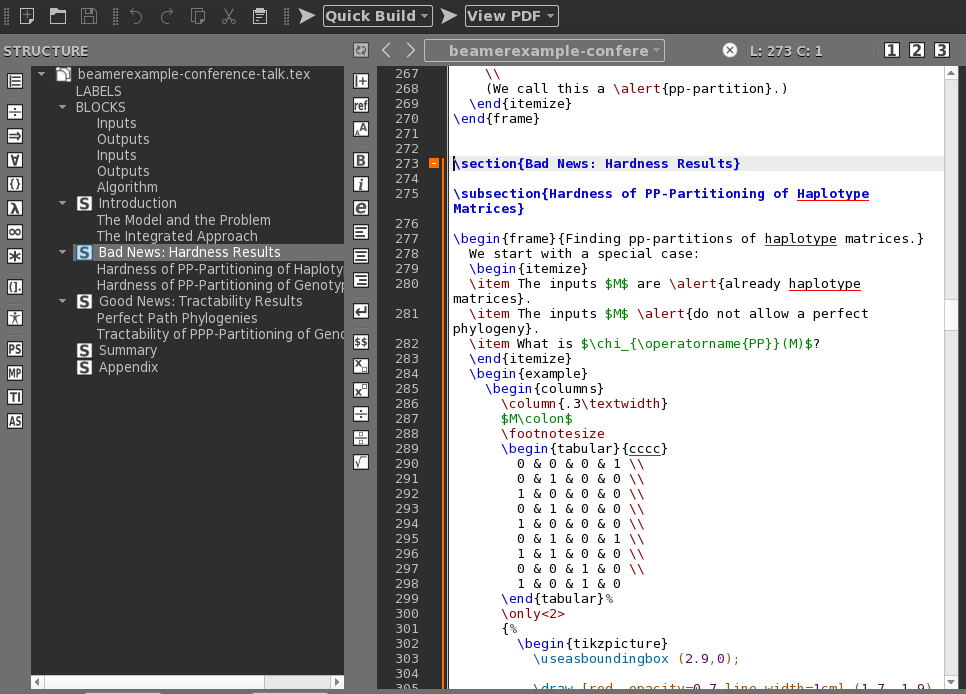
\includegraphics[width=0.99\linewidth]{../Norme_di_progetto/img/texMaker.png}
	\caption{\TeX{}maker - per la stesura dei documenti}
\end{figure}

\subsubsection{GanttProject}
GanttProject è un programma gratuito dedicato alla produzione dei diagrammi di Gantt\glo. Permette di creare task e milestone, organizzare le task in lavoro strutturato a interruzioni, disegnare
i vincoli di dipendenza tra di esse e molte altre utilità, generando automaticamente il relativo diagramma. \\
\centerline{\url{https://www.ganttproject.biz/}}
\begin{figure}[H]
	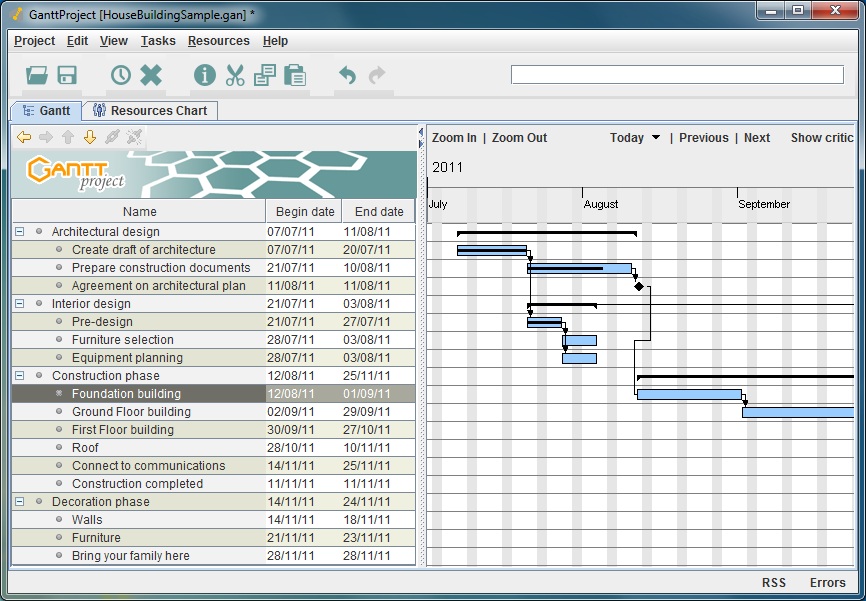
\includegraphics[width=0.99\linewidth]{../Norme_di_progetto/img/gantt.png}\\
			\caption{GanttProject - per la relizzazione di diagrammi di Gantt}
\end{figure}

\subsubsection{Draw.io}
Draw.io viene utilizzato per la produzione degli UML.\\
\centerline{\url{https://www.draw.io/}} 

\subsection{Gestione della configurazione}
L'obiettivo della configurazione è di creare ordine tra i documenti e il software. Tutto ciò che è configurato ha uno stato identificativo, è modificato secondo regole ben definite ed è posto sotto versionamento\glo.

\subsubsection{Versionamento}
\paragraph{Versionamento dei documenti} \mbox{} \\ \mbox{} \\
Ogni versione di qualsiasi documento deve corrispondere ad una riga della tabella delle modifiche. Il numero di versione è composto da tre cifre: \\ \\
\centerline{X.Y.Z} \\
\begin{itemize}
\item \textbf{X}: rappresenta una versione stabile del documento, resa tale dopo l'approvazione del \textit{Responsabile} di progetto: \begin{itemize}
\item inizia da 0 
\item viene incrementata di un'unità alla volta;
\end{itemize}
\item \textbf{Y}: indica l'ultima versione del documento che ha passato la fase di verifica: \begin{itemize}
\item inizia da 0;
\item viene incrementato dal verificatore ad ogni verifica;
\item quando viene incrementato X, viene riportato a 0.
\end{itemize} 
\item \textbf{Z}: indica l'ultima modifica apportata al documento dal redattore: \begin{itemize}
\item inizia da 0;
\item viene incrementato dal redattore del documento ad ogni modifica;
\item quando viene incrementato Y, viene riportato a 0.
\end{itemize}
\end{itemize}

\paragraph{GitHub} \mbox{} \\ \mbox{} \\
Per le parti del progetto da versionare si è scelto di usare GitHub\glo, un servizio del sistema di versionamento distribuito Git per contenere la repository remota. \\
I membri del team possono interagire con il VCS\glo sia da linea di comando, sia attarverso software che ne migliorano l'usabilità, come GitKraken e GitHub Desktop. La versione ufficiale del progetto è ospitata in una repository remota su GitHub, all'indirizzo \\
\centerline{\url{hhttps://github.com/teamafkSWE}}

\paragraph{Struttura del repository} \mbox{} \\ \mbox{} \\
All'interno della repository principale sopra descritta, ci sono due differenti repository: \begin{itemize}
\item \textbf{PredireConGrafana-docs}: contiene tutti i documenti ufficiali del progetto, suddivisi in specifiche cartelle: \\
\centerline{\url{https://github.com/teamafkSWE/PredireConGrafana-docs}}  \begin{itemize}
\item \textbf{Cartella principale - RR}: raccoglie i file sorgenti per la compilazione dei documenti, suddivisi tra esterni ed interni, realizzati per la \textit{Revisione dei Requisiti}. In futuro, saranno aggiunte cartelle distinte nominate \textbf{RP, RQ} e \textbf{RA}, contenenti i file delle rispettive consegne;
\begin{itemize}
\item[$\bullet$] \textbf{Tipologia\_di\_Documento}: ogni documento avrà la rispettiva cartella (e.i. Norme\_di\_Progetto), contenente tutti i file (sezioni ed immagini) necessari per la sua compilazione;
\item[$\bullet$] \textbf{copertina.tex}: file che permetterà una facile e rapida modifica dell'impostazione testuale del frontespizio;
\end{itemize}
\item \textbf{Template}: contiene tutti i file che definiscono il template \LaTeX{} per la creazione di nuovi documenti;
\end{itemize} 
\item \textbf{PredireConGrafana-SW}: conterrà tutti i file di codifica dei plug-in da sviluppare. \\ \centerline{\url{https://github.com/teamafkSWE/PredireConGrafana-SW}}
\end{itemize}
Entrambe le repository, avranno una propria struttura identica a livello: \begin{itemize}
\item \textbf{locale}: ogni membro del gruppo lavora sui file clonati dal repository remoto nel proprio PC;
\item \textbf{remoto}: presente su GitHub, contiene il lavoro svolto da ogni componente e che viene condiviso con il team.
\end{itemize}

\paragraph{Tipi di file} \mbox{} \\ \mbox{} \\
I file utilizzati per la documentazione del progetto sono: \begin{itemize}
\item file con estensione .tex di \LaTeX{};
\item file con estensione .pdf (da consegnare);
\item file di stile, .sty,  e immagini di supporto.
\end{itemize}
Il file ".gitignore" è presente al livello più esterno della repository ed elenca tutti i file esclusi dal versionamento.

\paragraph{Utilizzo di Git} \mbox{} \\ \mbox{} \\
Il repository di Git è composto da vari branch\glo, per favorire la collaborazione tra i vari membri e il parallelismo delle attività. Si consiglia quindi di seguire questa procedura:
\begin{enumerate}
\item scegliere il proprio branch di lavoro;
\item eseguire il pull\glo dal repository remoto, che effettua quindi l'aggiornamento del proprio repository locale;
\item svolgere il compito assegnato;
\item eseguire il comando di aggiunta (add) dei file nuovi o modificati da condividere all'area di staging\glo;
\item eseguire il comando di commit\glo dei file aggiunti, corredato da un messaggio che identifica il lavoro svolto;
\item eseguire il push\glo del commit sul repository remoto.
\end{enumerate}

\paragraph{Gestione delle modifiche}\mbox{} \\ \mbox{} \\
Tutti i membri del team possono modificare i file in ogni branch, ad eccezione del branch master, per il quale occorre richiedere una pull e ottenere l'approvazione di un altro membro.

\subsection{Gestione della qualità}
Lo scopo è di garantire che il prodotto e i servizi offerti rispettino gli obiettivi di qualità e che i bisogni del proponente siano soddisfatti. 

\subsubsection{Descrizione}
La gestione della qualità viene approfondita nel \textit{Piano di Qualifica}, dove sono descritte le modalità utilizzate per garantire la qualità nello sviluppo del progetto. In particolare: \begin{itemize}
\item sono presentati gli standard utilizzati;
\item sono individuati i processi\glo di interesse;
\item sono individuati gli attributi del software piè importanti per il progetto.
\end{itemize}
Per ogni processo vengono descritti: \begin{itemize}
\item gli obiettivi da perseguire;
\item le strategie da applicare;
\item le metriche da utilizzare.
\end{itemize}
L'obiettivo è quello di ottenere software e documentazione di qualità soddisfacente.

\subsubsection{Strumenti}
Gli strumenti utilizzati per la qualità sono:
\begin{itemize}
\item forniti dallo standard ISO-12207\footnote{ISO-12207: standard ISO per la gestione del ciclo di vita del software.};
\item le metriche.
\end{itemize}

\paragraph{Metriche} \mbox{} \\ \mbox{} \\
Le metriche sono distinte in tre categorie: processi, documentazione e codifica. Per ciascuna di esse si indica il motivo per cui è stata scelta e la procedura di calcolo.

\subparagraph{Classificazione}\mbox{} \\ \mbox{} \\
Le metriche rispetteranno la seguente notazione: \\
\centerline{\textbf{M[categoria][numero]}}
dove: \begin{itemize}
\item Categoria: indica la categoria della metrica, più precisamente:
\begin{itemize}
\item \textbf{P} per indicare le metriche dei processi;
\item \textbf{D} per indicare le metriche dei documenti;
\item \textbf{S} per indicare le metriche della codifica del software.
\end{itemize}
\item Numero: identifica in maniera univoca la metrica in ogni categoria, assume un valore intero a due cifre incrementale a partire da 1.
\end{itemize}
Se nelle formule di calcolo delle metriche è presente il simbolo "\#", va inteso come la parola "numero". Un esempio può essere il seguente:
\[ \#parole\_doc = numero\ di\ parole\ presenti\ nel\ documento \]
\pagebreak
\subparagraph{Metriche per i processi}  \mbox{} \\ 
\begin{table}[H]
\caption{Metriche dei processi}
	\begin{center}
	\begin{tabular}{ c | c | L{9.5cm} }
		\rowcolor{redafk}
		\textcolor{white}{\textbf{Nome}} & \textcolor{white}{\textbf{Codice}}& \centerline{\textcolor{white}{\textbf{Descrizione}}} \\
		Schedule Variance (SV)  & MP01 & La Schedule Variance indica se una certa attività o processo è in anticipo, in pari, o in ritardo rispetto alla data di scadenza prevista. \'E calcolata utilizzando la seguente formula: \newline
\[ SV = DCE-DCP\]
dove: \begin{itemize}
\item \textbf{DCE}: data conclusione effettiva;
\item \textbf{DCP}: data conclusione pianificata.
\end{itemize}
Se $SV \leq 0$ significa che l’attività o il processo è in pari o in anticipo, invece, se $SV > 0$ significa che l’attività è in ritardo. \\	
		Budget Variance (BV) & MP02 & Permette di controllare i costi sostenuti alla data corrente rispetto al budget preventivato. Viene calcolata in fase di consuntivo di periodo utilizzando la seguente formula: \newline
		\[ BV[\%] = \frac{CP-CE}{CE}\cdot 100 \]		
dove: \begin{itemize}
\item \textbf{CP}: costo preventivato;
\item \textbf{CE}: costo effettivo.
\end{itemize}
Se $BV[\%] \geq 0$ indica che il budget sta venendo speso più lentamente di quanto pianificato, se negativo invece indica che il budget sta venendo speso più velocemente di quanto pianificato. \\
Produttività (P) & MP03 & Rappresenta la produttività media delle risorse impiegate, cioè delle persone coinvolte, nelle diverse fasi del progetto. E’ misurata in termini di numero di linee di codice (\hyperref[par:MS01]{LOC}) sviluppate da una persona nell’unità di tempo stabilita (settimana). E’utilizzata per valutare lo sforzo richiesto per lo sviluppo  del progetto a fronte delle sue dimensioni. 
\[ Pmedia = \frac{LOC}{settimana}\]
	\end{tabular}
	\end{center}
	\end{table}
\pagebreak
\subparagraph{Metriche per i documenti}\mbox{} \\ 
\begin{table}[H]
\caption{Metriche dei documenti}
	\begin{center}
	\begin{tabular}{ c | c | L{10cm} }
		\rowcolor{redafk}
		\textcolor{white}{\textbf{Nome}} & \textcolor{white}{\textbf{Codice}} & \centerline{\textcolor{white}{\textbf{Descrizione}}} \\
		Indice Gulpease (IG)  & MD01 & \'E un indice di leggibilità di un testo tarato sulla lingua italiana e basato su due variabili linguistiche: la lunghezza della parola e la lunghezza della frase rispetto al numero delle lettere. La formula per il suo calcolo è: \newline
\[ IG = 89 + \frac{300 \cdot (\#frasi) - 10 \cdot (\#lettere)}{\#parole} \] \newline
Il risultato è un valore compreso nell'intervallo tra 0 e 100, dove il valore 100 indica la più alta leggibilità. Un indice inferiore a 80 indica documenti di difficile leggibilità per chi ha la licenza elementare, inferiore a 60 per chi ha la licenza media, inferiore a 40 per chi ha un diploma superiore.
	\\
	\end{tabular}
	\end{center}	
	\end{table}
\pagebreak
\subparagraph{Metriche per la codifica} \mbox{} \\ \mbox{} \\
Questa sezione ha lo scopo di fornire delle metriche per garantire un buon livello di qualità del software.
\begin{table}[H]
	\caption{Metriche del software}
	\begin{center}
	\begin{tabular}{ C{4.5cm} | c | L{9.5cm} }
		\rowcolor{redafk}
		\textcolor{white}{\textbf{Nome}} & \textcolor{white}{\textbf{Codice}} & \centerline{\textcolor{white}{\textbf{Descrizione}}} \\
		\label{par:MS01}Linee di Codice (LOC) & MS01 & Rappresenta  le  dimensioni  del  codice  sorgente  (di  tutto  il  prodotto  software oppure di quello sviluppato in una versione specifica). \'E espresso in termini di numero di linee di codice, ed è utilizzato per dimensionare la produttività delle persone e da questa lo sforzo richiesto per sviluppare il prodotto. \\
		Numero dei Metodi (NM)  & MS02 & Numero medio di metodi contenuti nelle classi di un oggetto. Un numero troppo alto di metodi può indicare la necessità di scomporre la classe. Un numero troppo basso deve far riflettere sull'effettiva utilità della classe in esame. 
		\[ NM =\frac{\sum\#metodi}{\#classi}  \] \\
		Numero di Parametri (NP) & MS03 & Numero di parametri passati a un metodo. Un eccessivo numero di parametri passati ad un metodo può
indicare un’eccessiva complessità dello stesso. \\
		Commenti per Linee di \newline Codice (CLC) & MS04 & Rapporto fra numero di righe di commento e numero totale di righe (vuote escluse). Un codice ben commentato può essere compreso più facilmente e velocemente, facilitando le operazioni di manutenzione. 
		\[ CLC = \frac{\#righe\_commento}{\#tot\_righe}\] \\
		Code Coverage (CC) & MS05 & Percentuale delle linee di codice coperte dai test. Avere codice coperto da test riduce la possibilità di introdurre errori nel prodotto. 
		\[ CC[\%] = \frac{\#righe\_codice\_testate}{\#tot\_righe\_codice}\] \\
	\end{tabular}
	\end{center}
	\end{table}
\pagebreak
\subsubsection{Verifica}
Il processo di verifica ha come scopo la realizzazione di prodotti corretti, coesi e completi. Sono soggetti a verifica i documenti e il software.
Il processo di verifica deve rispettare i seguenti punti: \begin{itemize}
\item la verifica deve essere effettuata seguendo procedure ben definite;
\item per verificare vi sono criteri chiari e affidabili;
\item ogni fase del prodotto viene verificata;
\item dopo la verifica il prodotto è in uno stato stabile;
\item il prodotto può essere validato.
\end{itemize}
Il processo di verifica prende in input ciò che è già stato prodotto e lo restituisce in uno stato
conforme alle aspettative (stabile). Per ottenere tale risultato ci si affida a processi di analisi e test.
\paragraph{Strumenti di verifica}

\paragraph*{Correzione ortografica} \mbox{} \\ \mbox{} \\
Il controllo ortografico viene eseguito principalmente basandosi sugli strumenti integrati in \TeX{}maker, il quale fornisce un dizionario italiano e sottolinea in rosso le parole che non vi appartengono. 

\paragraph{Analisi} \mbox{} \\ \mbox{} \\
Il processo di analisi si suddivide in statica e dinamica.

\paragraph*{Analisi statica} \mbox{} \\ \mbox{} \\
L'analisi statica effettua controlli su documenti e codice. Questo tipo di analisi serve per rilevare varie tipologie di anomalie. \\
Questa attività viene effettuata con l'ausilio di due metodi manuali di lettura (attuati da persone) differenti: \begin{itemize}
\item \textbf{Walkthrough}: i vari componenti del team effettuano una lettura scrupolosa di documenti e/o codice alla ricerca di errori, senza sapere inizialmente se ce ne siano;
\item \textbf{Inspection}: i verificatori usano liste di controllo (checklist) per fare ispezione cercando errori specifici in parti specifiche. Questa tecnica permette quindi di aumentare l'efficienza dello sviluppo, diminuendo i tempi dell'analisi statica.
\end{itemize}
A seguire sono descritte le liste di controllo utilizzabili per le ispezioni:
\begin{table}[H]
\caption{Errori frequenti nei documenti}
\begin{center}
\begin{tabular}{C{4cm} | C{12cm}}
\rowcolor{redafk}
\textcolor{white}{\textbf{Oggetto}} & \centerline{\textcolor{white}{\textbf{Controllo}}} \\
Formato data & Deve seguire il formato gregoriano YYYY-MM-DD \\
Sintassi & La frase è troppo complessa e deve essere semplificata \\
Punteggiatura degli elenchi & Ogni voce termina in ";" eccetto l'ultima che termina in "."\\
Errori di battitura & Tipici errori di battitura dovuti alla vicinanza delle
lettere sulla tastiera, ad esempio la lettera "a" al posto della "s", "i" al posto di "o", "m" al posto di "n" \\
Gerarchia delle sezioni & Non viene scritta la gerarchia delle sezioni dei documenti in maniera adeguata, ovvero: section, subsection, subsubsection, paragraph, subparagraph
\end{tabular}
\end{center}
\end{table}

\paragraph*{Analisi dinamica} \mbox{} \\ \mbox{} \\
L'analisi dinamica è una tecnica di analisi del prodotto software che richiede la sua esecuzione. Produce una misura della qualità del prodotto, mediante l'esecuzione di test specifici che verificano se il prodotto funziona e se ci sono anomalie.

\paragraph{Test} \mbox{} \\ \mbox{} \\
I test sono l'attività fondamentale dell'analisi dinamica: il loro scopo è verificare che il codice
scritto funzioni correttamente. I test devono:
\begin{itemize}
\item essere ripetibili;
\item specificare l'ambiente di esecuzione;
\item identificare input e output richiesti;
\item avvertire di possibili effetti indesiderati;
\item fornire informazioni sui risultati dell'esecuzione.
\end{itemize}
Ci sono vari tipi di test, ognuno dei quali ha un diverso oggetto di verifica e scopo.

\paragraph*{Test funzionali} \mbox{} \\ \mbox{} \\
Test condotti per valutare la conformità di un componente o sistema con requisiti\glo funzionali. Ne fanno parte: \begin{itemize}
\item \textbf{Test di unità\glo}: si eseguono su unità di software, e si concentrano sul loro funzionamento individuale;
\item \textbf{Test di integrazione}: verificano se sono rispettati i contratti di interfaccia tra più moduli o sub-system (interni o esterni);
\item \textbf{Test di accettazione UAT}: gli UAT (User Acceptance Testing) si occupano di verificare il prodotto e, in particolare, il soddisfacimento del cliente. Il superamento di questo test garantisce che il software sia pronto per essere rilasciato.
\end{itemize}

\paragraph*{Test di regressione} \mbox{} \\ \mbox{} \\
Il test di regressione va eseguito ogni volta che viene modificata un’implementazione in un programma. È possibile eseguire nuovamente i test esistenti sul codice modificato, integrando solo le parti che abbiano precedentemente superato il test di unità, per stabilire se le modifiche apportate hanno alterato elementi precedentemente funzionanti.\\ Se necessario è anche possibile scrivere nuovi test.

\paragraph*{Test di sistema} \mbox{} \\ \mbox{} \\
Verificano il comportamento dell'intero sistema.\\
Lo scopo principale di questi test è la verifica del sistema rispetto alle specifiche tecniche definite nell'\textit{Analisi dei Requisiti}.

\subsubsection{Validazione}
Questo processo avviene tramite test pianificati dal \textit{Progettista} ed in seguito eseguiti dal \textit{Verificatore}.
Lo scopo di quest'ultimi è appunto accertare che il prodotto finale corrisponda alle attese, soddisfando tutti i requisiti concordati e i bisogni del committente. \\
Tali test sono soggetti a tracciamento e verranno riportati all'interno del \textit{Piano di Qualifica}.
